\documentclass{article}
\usepackage[spanish]{babel}
\usepackage[utf8]{inputenc}
\usepackage{graphicx}
\usepackage{minted}

\title{\textbf{Criptografía aplicada: Cálculo del hash SHA-256 de un bloque Bitcoin}}
\author{Javier Domínguez Gómez \\
\small{jdg@member.fsf.org} \\
\small{Fingerprint: 94AD 19F4 9005 EEB2 3384 C20F 5BDC C668 D664 8E2B}}
\date{v0.1.03 - Febrero 2019}

\begin{document}
\maketitle

\tableofcontents{}

\section{Introducción}
    Este documento describe en detalle las partes de la cabecera de un bloque cualquiera en la cadena de bloques de Bitcoin, así como las operaciones lógico-matemáticas de la función criptográfica SHA-256 que se emplean con el fin de generar el \textit{hash} adecuado que finalmente representará dicho bloque en la cadena de bloques.
    
    \vspace{3mm}
    En primer lugar se ha de tener en cuenta que cada bloque de la cadena de bloques de Bitcoin contiene una cantidad considerable de información almacenada en una estructura de datos compleja que se puede categorizar en la siguiente tabla.
    \begin{table}[H]
    \centering
    \begin{tabular}{| c | l | c | l |} 
        \hline
        Tipo de dato & Nombre & Tamaño & Descripción \\
        \hline
        $uint32_t$ & magicID & 4 bytes & Valor constante 0xD9B4BEF9.\\
        \hline
        $uint32_t$ & headerLenght & 4 bytes & Logitud del bloque.\\
        \hline
        $uint32_t$ & versionNumber & 4 bytes & Valor variable, actualmente 2.\\
        \hline
    \end{tabular}
    \caption{\textit{Datos de la cabecera de un bloque en la cadena de bloques de Bitcoin.}}
    \label{table:2}
    \end{table}
    
    \begin{figure}[H]
    \centering
        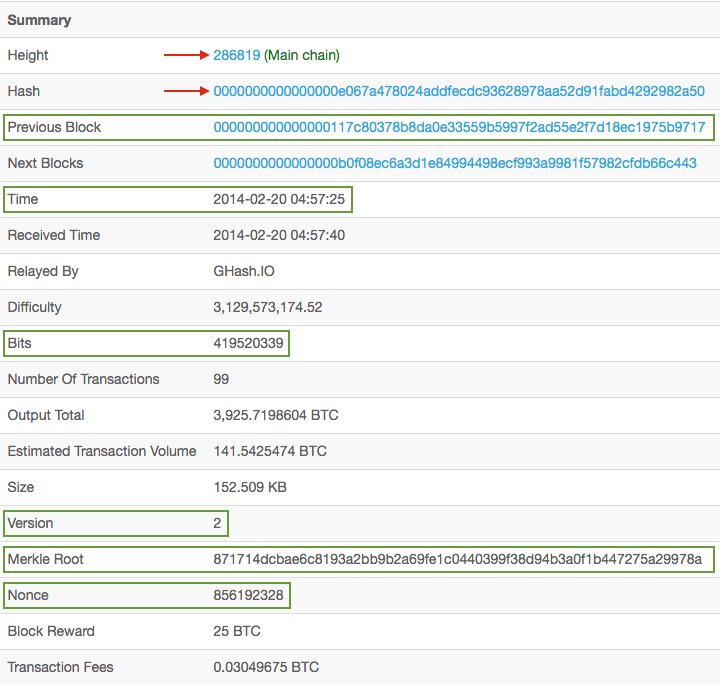
\includegraphics[scale=0.47]{img/Bitcoin_block_SHA_256_Block_Data}
        \caption{Datos empleados para la obtención del \textit{hash} del bloque $286819$.}
    \end{figure}
    
    \vspace{3mm}
    En la siguiente figura se detalla el contenido de los primeros 16 registros de la variable $W_{t}$ en cada una de las tres veces que se ejecutan las 64 iteraciones de la función SHA-256 para obtener el \textit{digest} en cada caso.
    \begin{figure}[H]
    \centering
        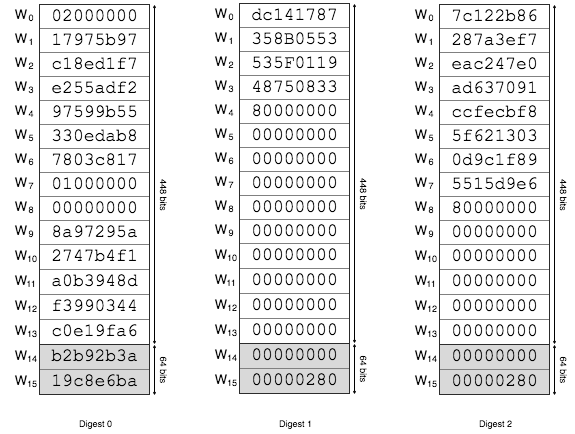
\includegraphics[scale=0.59]{img/Bitcoin_block_SHA_256_W0_W15_x3}
        \caption{Los primeros 16 registros de la variable $W_{t}$ en los tres casos en los que se ha de ejecutar la función SHA-256.}
    \end{figure}
\section{Fecha en formato Unix}
    \begin{figure}[H]
    \centering
        \begin{minted}{c}
    #include <stdio.h>
    #include <time.h>
    
    int main(int argc, char *argv[]) {
    
    	int year, month, day, hour, minute, second;
    	struct tm t;
    	time_t tod;
    
    	printf("Year: ");
    	scanf("%d", &year);
    	printf("Month: ");
    	scanf("%d", &month);
    	printf("Day: ");
    	scanf("%d", &day);
    	printf("Hour: ");
    	scanf("%d", &hour);
    	printf("Minute: ");
    	scanf("%d", &minute);
    	printf("Second: ");
    	scanf("%d", &second);
    
    	t.tm_year = year - 1900;
    	t.tm_mon = month - 1;   // Values [0-11]
    	t.tm_mday = day;
    	t.tm_hour = hour + 1;   // GMT+1
    	t.tm_min = minute;
    	t.tm_sec = second;
    	t.tm_isdst = 0;         // DST = 0
    	tod = mktime(&t);
    
    	printf("Timestamp epoch: %ld\n", (long) tod);
    }
        \end{minted}
    \end{figure}

\end{document}
